\documentclass{article}
\usepackage[headheight=40pt, textheight=560pt]{geometry}
\usepackage{paralist}
\usepackage{scalerel,amssymb}
\usepackage{amsmath}
\usepackage{colortbl}
\usepackage{array}
\usepackage{multirow}
\usepackage{blindtext}
\usepackage{reledmac}
\usepackage{changepage}

\usepackage{pgfplots}
\usepackage{tikz}
\usetikzlibrary{positioning}
\usetikzlibrary{shapes.geometric, arrows}
\tikzstyle{arrow} = [thick,->,>=stealth]

\usepackage{graphicx}
\usepackage{stix}

\newcommand{\tableflip}{$($\rotatebox{45}{$\smile$}$^{\circ}\smwhtsquare^{\circ})\rotatebox{45}{$\smile$}\mkern-6mu\frown$\raisebox{0.5ex}{$\bot$}$\mkern-3.5mu-\mkern-3.5mu$\raisebox{0.5ex}{$\bot$}}

\usepackage{stackengine}
\def\apeqA{\SavedStyle\sim}
\def\apeq{\setstackgap{L}{\dimexpr.5pt+1.5\LMpt}\ensurestackMath{%
  \ThisStyle{\mathrel{\Centerstack{{\apeqA} {\apeqA} {\apeqA}}}}}}

\usepackage{fancyhdr}
\fancyhead[L]{
	\begin{tabular}{ll}
		\begin{tabular}{l}
			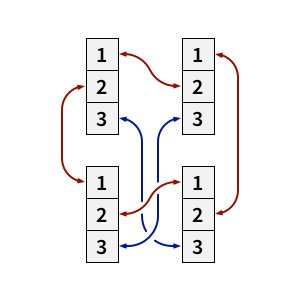
\includegraphics[scale=0.13]{distributed}
		\end{tabular}	
		&
		\begin{tabular}{l}
			\LARGE \textbf{Distributed Algorithms} \\
			\Large \textsc{Summary}
		\end{tabular}
	\end{tabular}
}
\fancyhead[R]{
	\begin{tabular}{r}
		16-124-836 \\
		Marcel \textsc{Zauder}
	\end{tabular}
}
\renewcommand{\headrulewidth}{0.4pt}
\fancyfoot[L]{\hspace{2cm}\thepage}
\fancyfoot[C]{}
\fancyfoot[R]{Designing Data-Intensive Application}
\renewcommand{\footrulewidth}{0.4pt}

\usepackage{hyperref}

\begin{document}
	\pagestyle{fancy}
	\section{Reliable, Scalable, and Maintainable Applications}
	\begin{adjustwidth}{2em}{2em}
		\textit{Introduces the terminology and approach that we're going to use throughout this book. It examines what we actually mean by words like \textbf{reliability}, \textbf{scalability}, and \textbf{maintainability}, and how we can try to achieve these goals.}
		\subsection{Thinking about Data Systems}
		\begin{adjustwidth}{2em}{2em}
			Because nowadays most applications are \textit{data-intensive}, as opposed to \textit{compute-intensive}, the raw CPU power is rarely a limiting factor for these. The bigger problems are usually the amount and the complexity of data and the speed at which it is changing. So often the following specifications are necessary for many applications: \\
			\begin{adjustwidth}{1em}{1em}
				\begin{enumerate}[\footnotesize{\textbullet}]
					\item The storage of data should be so that they, or another application which will use it, can find it easily (\textit{databases})
					\item Remember the results of an expensive operation, to speed up reads (\textit{caches})
					\item Users can search the databases by keyword or filter in various ways (\textit{search indexes})
					\item The system can be handled asynchronously by sending a message to another process (\textit{stream processing})
					\item Periodically crunch a large amount of accumulated data (\textit{batch processing})
				\end{enumerate}
			\end{adjustwidth}
			\hfill \\
			The usage of databases is very common and therefore these functionalities sound plainfully obvious. When designing and engineering a new application databases are a perfectly good tool instead of always creating a new data storage engine from scratch.
		\end{adjustwidth}
		\subsection{Reliable}
		\begin{adjustwidth}{2em}{2em}
		\end{adjustwidth}
	\end{adjustwidth}
	
	
	\newpage\null\thispagestyle{empty}
	\newpage
	\setcounter{section}{0}
	
	
	\fancyfoot[R]{
		Introduction to Reliable and Secure Distributed Programming
	}
	\section{Introduction}
	\begin{adjustwidth}{2em}{2em}
	\end{adjustwidth}
	
	
	\newpage\null\thispagestyle{empty}
	\newpage
	\setcounter{section}{0}
	
	
	\fancyfoot[R]{
		Additional Literature \\
		Defining Dependable Systems
	}
	\section{Terminology}
	\begin{adjustwidth}{2em}{2em}
	\end{adjustwidth}
	
\end{document}